\section{Model Exercise 0-1b (01): Bending fracture test (OPA)}
\label{sec:mex01b}
\Authors{Amir Sattari, Keita Yoshioka}

\subsection{Experimental set-up and results}

In this model exercise, the effect of the anisotropy on the fracture toughness of the Opalinus claystones experimentally and numerically is investigated. The description of the experimental setup and the test procedure is explained in section \ref{sec:Fracture_Toughness_Exp}, where a fracture toughness test on a sample with the dimension of 140x30x30 $(mm)$ $(LxWXT)$ is carried out. The notch dimension is 2x10x30 $(mm)$ $(LxWXT)$ and the span length is 120 $mm$. The anisotropy of a claystone depends mainly on the orientation of the embedded layers. When the loading direction is perpendicular ($\bot$) to the layering orientation the materials strength is highest. In contrast, when the loading direction is parallel ($\parallel$) to the layering orientation, the materials strength is the lowest. The peak load attained from the experimental data ($\bot$) is 598 $N$ and the bending stiffness is around 3.3 $GPa$ (Figure \ref{fig:Amir_Fracture_Toughness_Result_20}). The crack mouth opening before the failure is 24 $\mu m$. The 4K video with the 30fps is used to track the reference points on the claystone. Afterward, the image analyzing technique is implemented to determine the CMOD. The 30fps video was not able to detect the brittle failure of the sample and therefore in the experimental data, the post failure response is not well represented. The measured fracture toughness ($\bot$) is $0.746\ MPa.\sqrt\ m$. The anisotropy effect of claystone is observed based on the fracking pattern of different samples under mechanical loading without temperature and humidity control (Figure \ref{fig:Amir_Fracture_Toughness_Fracture_a}). The propagation of fracks parallel to the layering orientation, where the sample is weakest, is observed (Figure \ref{fig:Amir_Fracture_Toughness_Fracture_b}). Similarly, inside the climate chamber, and under 50 and 80 $^{\circ}C$ temperature conditions, the fracture toughness of the claystone is measured ( Table \ref{table:Amir_Fracture_Toughness_Table1}).

\begin{figure}[!ht]
\centering
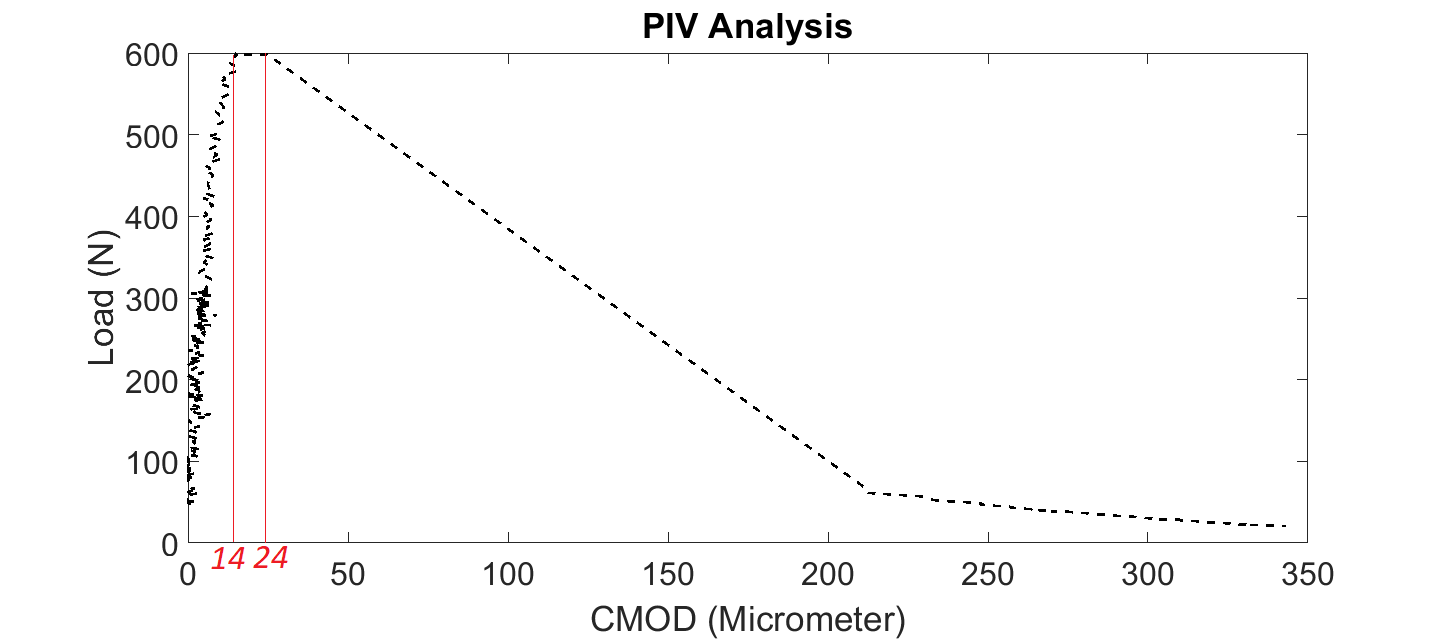
\includegraphics[width=11cm,height=5cm]{figures/Amir_Fracture_Toughness_Result_20.png}
\caption{The load vs. CMOD for the Opalinus claystone sample under the room temperature}
\label{fig:Amir_Fracture_Toughness_Result_20}
\end{figure}

\begin{figure}[!ht]
\centering
\begin{subfigure}[c]{0.43\textwidth}
\centering
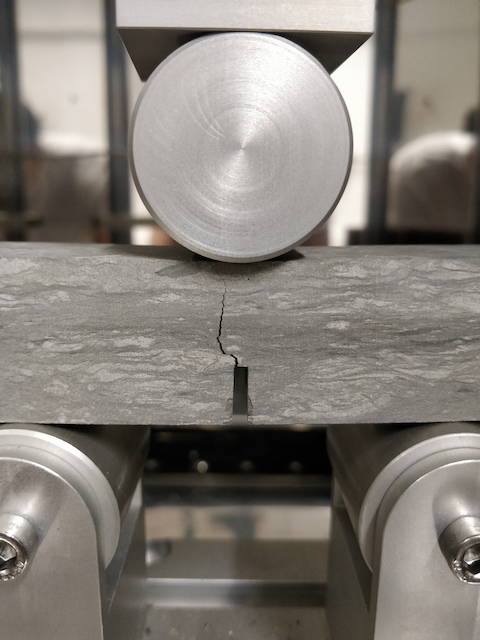
\includegraphics[width=4cm,height=5cm]{figures/Amir_Fracture_Toughness_Fracture_a.png}
\subcaption{}
\label{fig:Amir_Fracture_Toughness_Fracture_a}
\end{subfigure}
\hfill
\begin{subfigure}[c]{0.55\textwidth}
\centering
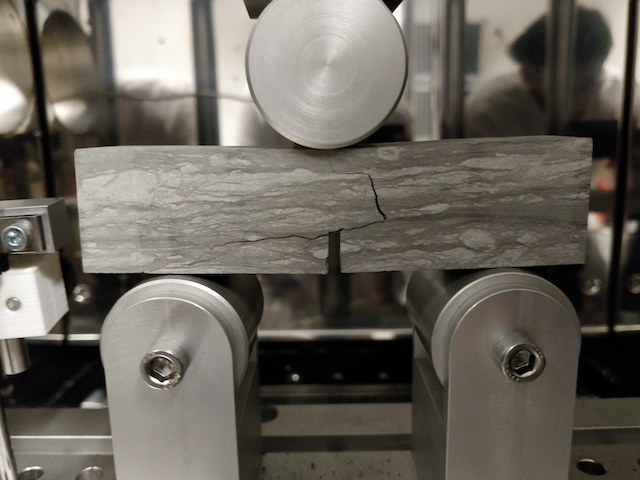
\includegraphics[width=6cm,height=5cm]{figures/Amir_Fracture_Toughness_Fracture_b.png}
\subcaption{}
\label{fig:Amir_Fracture_Toughness_Fracture_b}
\end{subfigure}
\caption{The anisotropy of the frack propagation in claystone (a) the frack propagation parallel to the loading direction, (b) the frack propagation through the weak interface}
\end{figure}

\begin{table}[!ht]
\centering
\begin{center}
\begin{tabular}{ | >{\centering\arraybackslash}X m{14em} | >{\centering\arraybackslash}X m{5em}| >{\centering\arraybackslash}X m{5em} |
>{\centering\arraybackslash}X m{5em} |} 
\hline
Test Results & 20$^{\circ}C$ & 50$^{\circ}C$ & 80$^{\circ}C$ \\
\hline
Peak Force ($N$) & 559 & 482 & 455 \\ 
\hline
Fracture Toughness $MPa.\sqrt m$. & 0.697 & 0.601 & 0.582\\
\hline
\end{tabular}
\end{center}
\caption{The Fracture toughness under different temperature conditions}
\label{table:Amir_Fracture_Toughness_Table1}
\end{table}


\subsection{Model approach}

\subsubsection*{Lattice-Element-Model (LEM)}

The LEM is implemented to investigate the anisotropy of claystone in two cases, where the loading direction is parallel or perpendicular to the layering orientation. The LEM setup ($\bot$) is generated in 2D with the back calculation of the outputs from the fracture toughness \ref{sec:Fracture_Toughness_Exp} and splitting \ref{sec:Brazilian_Disk_Exp} experimental results. The materials strength in perpendicular direction is considered to be 5 times higher than parallel case. The fracture paths for both ($\bot$) and ($\parallel$) cases are shown in Figure \ref{fig:Amir_ME1_LEM_Perpendicular} and \ref{fig:Amir_ME1_LEM_Parallel}, respectively. Figure \ref{fig:Amir_ME1_LEM_Claystone} illustrates the comparison between the experimental and numerical data. As discussed before, the post failure behavior does not match due to the experimental shortage of capturing the true load-displacements.


\begin{figure}[!ht]
\centering
\begin{subfigure}[b]{0.55\textwidth}
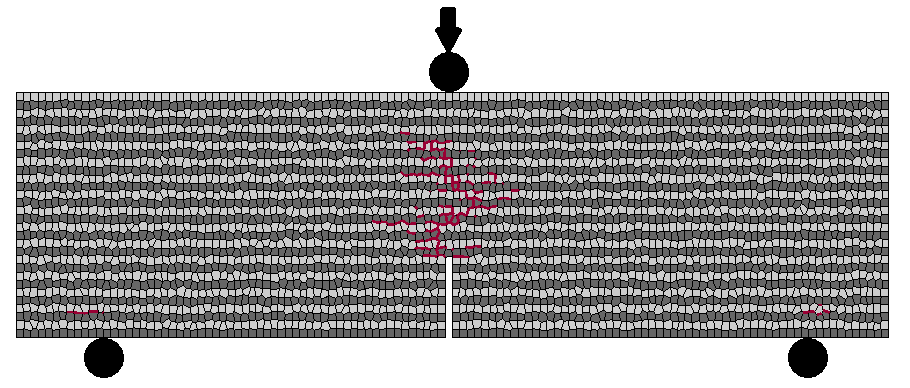
\includegraphics[width=1\linewidth]{figures/Amir_ME1_LEM_Perpendicular.png}
\subcaption{}
\label{fig:Amir_ME1_LEM_Perpendicular}
\end{subfigure}
%\hfill
\begin{subfigure}[b]{0.55\textwidth}
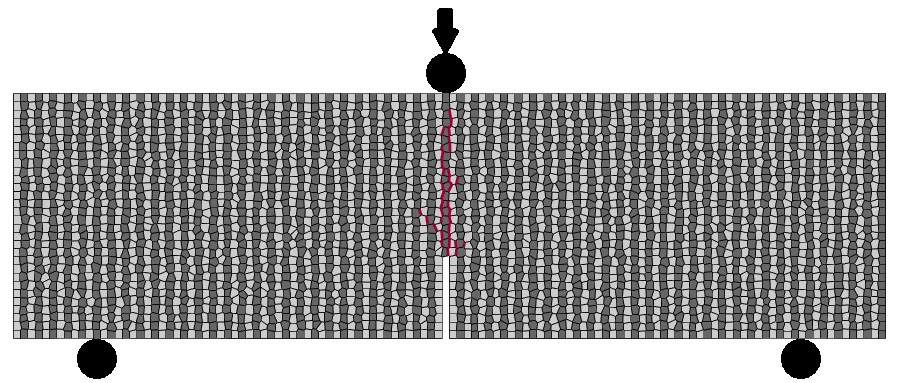
\includegraphics[width=1\linewidth]{figures/Amir_ME1_LEM_Parallel.png}
\subcaption{}
\label{fig:Amir_ME1_LEM_Parallel}
\end{subfigure}
\caption{The fracking path under loading direction (a) perpendicular, and (b) parallel to the layering orientation}
\end{figure}

\begin{figure}[!ht]
\centering
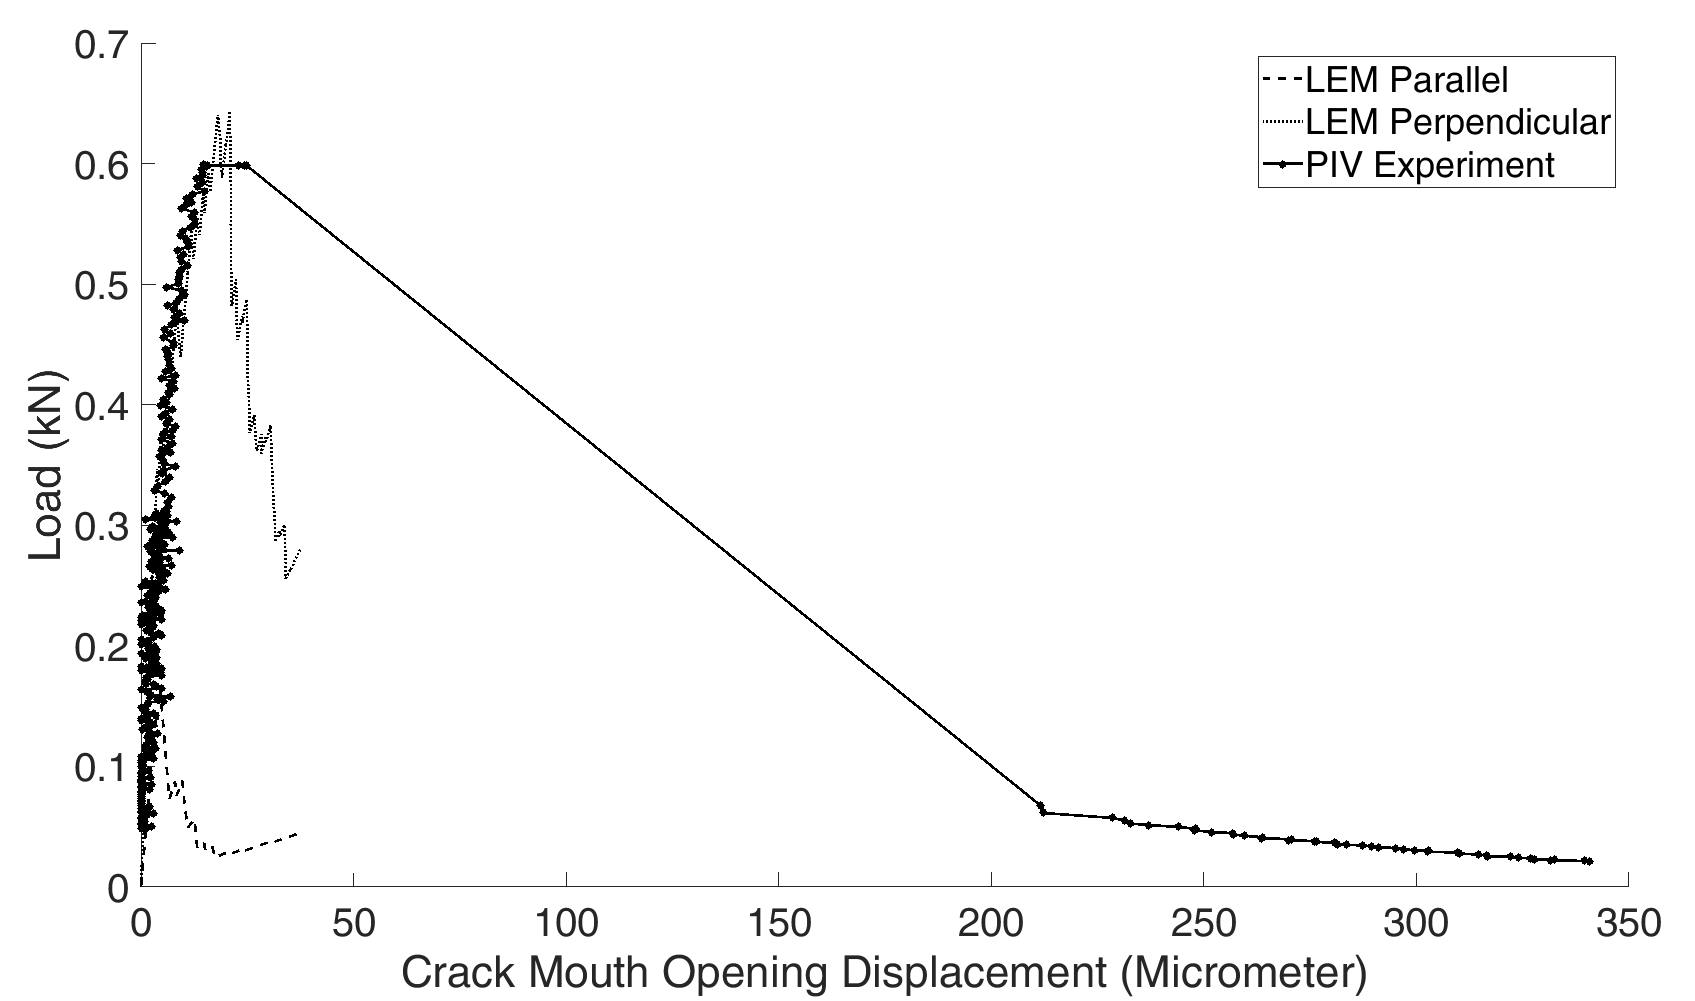
\includegraphics[width=0.75\textwidth]{figures/Amir_ME1_LEM_Claystone.png}
\caption{The comparison of experimental and numerical data for effect of anisotropy in Opalinus claystone} 
\label{fig:Amir_ME1_LEM_Claystone}
\end{figure}

\subsubsection*{Finite-Element-Approach: Variational Phase-Field (VPF)}

Extended experiment: parallel to the lamination Fig.~\ref{fig:ME1_ext_vpf_para_init} and orthogonal to the lamination Fig.~\ref{fig:ME1_ext_vpf_orth_init}.
Fracture simulation results are in Figs.~\ref{fig:ME1_ext_vpf_para_result} and~\ref{fig:ME1_ext_vpf_orth_result}, and the force vs. CMOD is in Fig~\ref{fig:ME1_ext_vpf_FvsCMOD}.

\begin{figure}[!ht]
\centering
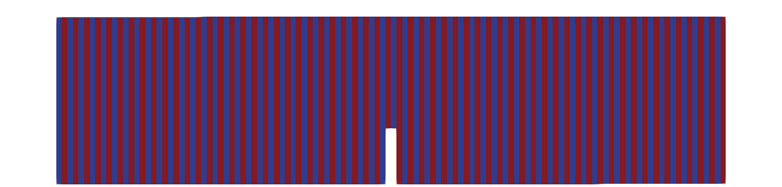
\includegraphics[width=1\textwidth]{figures/ME1_ext_2D_parallel_init.png}
\caption{Sample for parallel to the lamination}
\label{fig:ME1_ext_vpf_para_init}
\end{figure}

\begin{figure}[!ht]
\centering
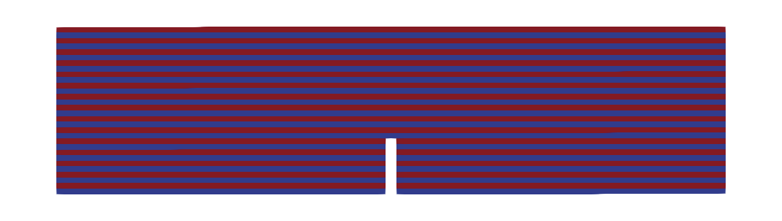
\includegraphics[width=1\textwidth]{figures/ME1_ext_2D_orthogonal_init.png}
\caption{Sample for orthogonal to the lamination}
\label{fig:ME1_ext_vpf_orth_init}
\end{figure}

\begin{figure}[!ht]
\centering
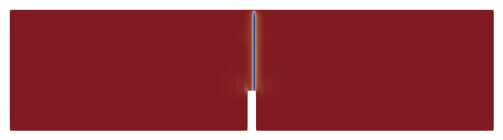
\includegraphics[width=1\textwidth]{figures/ME1_ext_2D_para_result.png}
\caption{Result of parallel to the lamination}
\label{fig:ME1_ext_vpf_para_result}
\end{figure}

\begin{figure}[!ht]
\centering
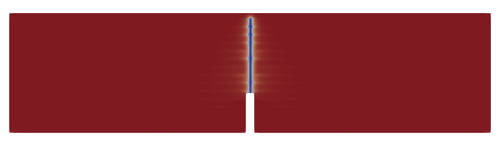
\includegraphics[width=1\textwidth]{figures/ME1_ext_2D_orth_result.png}
\caption{Result of orthogonal to the lamination}
\label{fig:ME1_ext_vpf_orth_result}
\end{figure}

\begin{figure}[!ht]
\centering
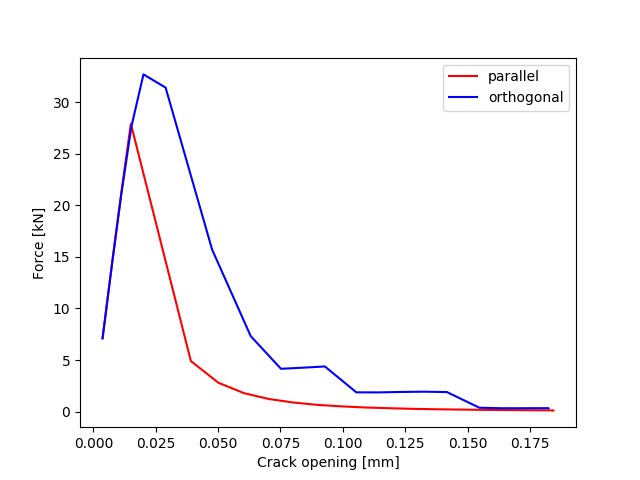
\includegraphics[width=1\textwidth]{figures/ME1_ext_NFvsCMOD.png}
\caption{Force vs. CMOD}
\label{fig:ME1_ext_vpf_FvsCMOD}
\end{figure}

\todo[inline]{[UFZ](KY): Description of OGS-VPF results}

\subsubsection{Results and discussion}

The lattice model is able to capture the existing anisotropy in the Opalinus claystone material. The fracking path dependence on the orientation of the embedded layers is shown in Figure \ref{fig:Amir_ME1_LEM_Perpendicular} and \ref{fig:Amir_ME1_LEM_Parallel}, which matches the experimental data given in Figure \ref{fig:Amir_Fracture_Toughness_Fracture_b}. Due to the layering orientation and stress distributions (in $\bot$ case), the fracking path has zigzag pattern following the weakest interface bonds. This irregularity of the frack path is not captured in VPF model. As mentioned before, the post failure results do not match experimental data due to the experimental tests limitation. The lattice model is validated with the experimental data exist for the ($\bot$) case and is extended to model the ($\parallel$) case, where the loading direction is parallel to the embedded layers. According to the Figure \ref{fig:Amir_Fracture_Toughness_Fracture_a}, the frack path is a straight line through the weak interface bond. More investigation needs to be done to determine and investigate the Opalinus claystone fracture toughness under different loading to the embedded layers orientation and the effect of the humidity and temperature on the fracture toughness. Additionally, the quantitative comparison of the results both for lattice and VPF models should be carried out.

\todo[inline]{Amir: Keita please write few sentences regarding your numerical part (Discussion)}

\todo[inline]{[CAU/UFZ](AS/KY): Short comparison of results}